% \usetikzlibrary{angles,quotes}

\section{Μοντελοποίηση Φορτίων Ελίκων}
\label{sec:prop}
\noindent Για την μοντελοποίηση των φορτίων της έλικας, αρχικά υποθέτουμε μία 
έλικα διαμέτρου \(D\), και με γωνιακή ταχύτητα περιστροφής \(\omega\). Η 
περιστροφική κίνηση, που εκτελεί η έλικα, παράγει μία δύναμη ώθησης \(T\), η 
οποία είναι κάθετη στο επίπεδο περιστροφής της έλικας, και μία ροπή \(N\), που 
επιδρά στον άξονα περιστροφής της έλικας. Για τον υπολογισμό των παραπάνω 
μεγεθών ακολουθείται η θεωρία στοιχειωδών πτερυγίων (\tl{Blade Element Theory}) 
\cite{Bose2012}. 
Σύμφωνα με το θεώρημα, τα πτερύγια της έλικας αποτελούνται από άπειρα, 
λεπτόπαχα, ανεξάρτητα, αεροδυναμικά στοιχεία, τα οποία είναι τοποθετημένα 
διαμήκους της ακτίνας της έλικας. Παίρνουμε μία αεροτομή πάχους \(dr\), με
\(r\) απόσταση από τον άξονα περιστροφής της έλικας. Στο σχήμα (\ref{blade}) 
φαίνονται οι δυνάμεις που ασκούνται στην αεροτομή: οπισθέλκουσα \(dD\), άντωση 
\(dL\). Η γωνία, που σχηματίζεται μεταξύ των ζευγών δυνάμεων \(dT\), \(dQ\) και 
\(dL\), \(dD\), ονομάζεται ολική γωνία κατωρεύματος \(\xi\). 

\begin{figure}[htb!]
    \centering
    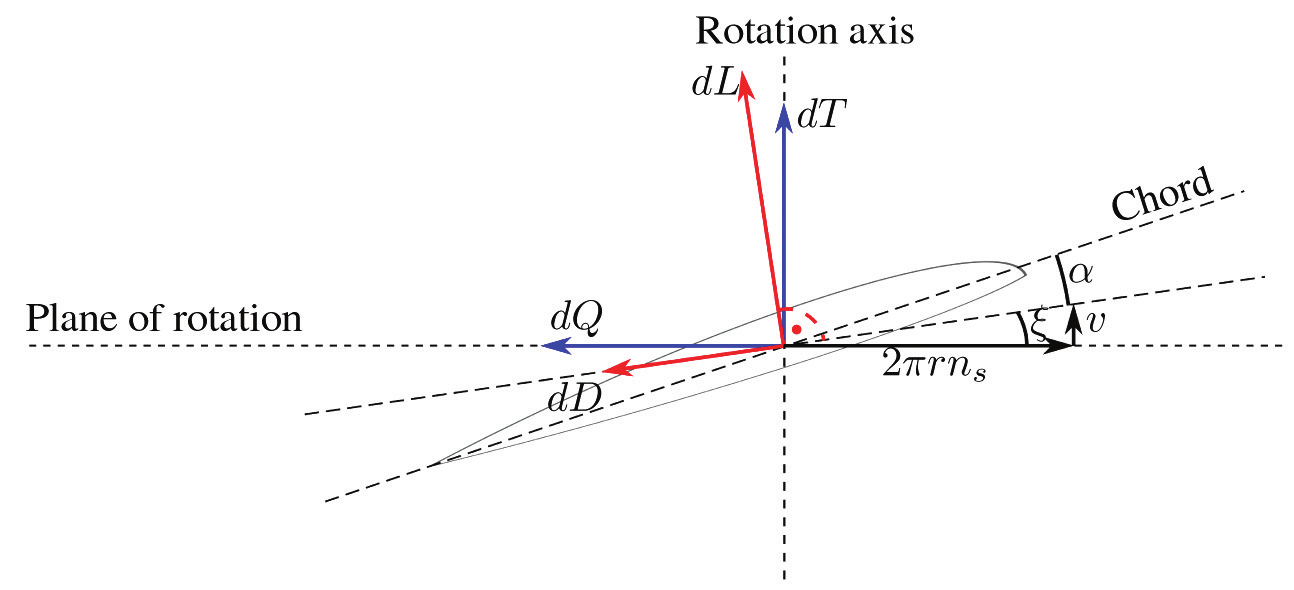
\includegraphics[width=\textwidth]{Propeller/blade_image.png}
    \caption{Διάγραμμα \tl{Blade Element Theory} \cite{automat}.}\label{blade}
\end{figure}

Σύμφωνα με το σχήμα (\ref{blade}), η στοιχειώδης δύναμη ώθησης \(dT\) και η 
στοιχειώδης δύναμη αντίστασης \(dQ\) υπολογίζονται βάσει της άντωσης και 
οπισθέλκουσας ως εξής

\begin{gather*}
    \mathrm{d}T = \mathrm{d}L \cos(\xi) - \mathrm{d}D \cos(\xi)\\
    \mathrm{d}Q = \mathrm{d}L \sin(\xi) + \mathrm{d}D \sin(\xi),
\end{gather*}
όπου οι δυνάμεις \(dL\) και \(dD\) εκφράζονται από τις σχέσεις
\begin{gather*}
    \mathrm{d}L = \frac{1}{2} \rho V_{e}^2 l c_L  \mathrm{d}r\\
    \mathrm{d}D = \frac{1}{2} \rho V_{e}^2 l c_D  \mathrm{d}r
\end{gather*}
\begin{conditions}
    V_e    &  την ενεργό ακτινική ταχύτητα\\
    l      &  το μέσο μήκος χορδής\\
    c_{D}  &  το συντελεστή οπισθέλκουσας\\
    c_{L}  &  το συντελεστή άντωσης\\
    \rho   &  την πυκνότητα αέρα.
\end{conditions}

Για να υπολογιστούν οι \(T\) και \(N\) για όλη την έλικα, παίρνουμε τα 
ολοκληρώματα σε όλη την επιφάνεια των πτερυγίων της ως
\begin{gather*}
    T = n_P \int_0^{R}\mathrm{d}T\,\mathrm{d}r \\
    N = n_P \int_0^{R}r\mathrm{d}Q\,\mathrm{d}r
\end{gather*}
\begin{conditions}
    n_P & τον αριθμό πτερυγίων έλικας \\
    R   & την ακτίνα έλικας.
\end{conditions}

Η ολοκλήρωση των παραπάνω δύο σχέσεων διατυπώνεται αναλυτικά στο \cite{Bose2012}.
Το αποτέλεσμα της ολοκλήρωσης είναι
\begin{equation*}
    \left. \begin{aligned}
        T &= C_T \rho D^4 n^2  \\
        N &= C_N \rho D^5 n^2  
    \end{aligned}
    \right. \qquad \text{με} \,\, n \,\, \text{ταχύτητα περιστροφής σε \tl{Hz}.}
\end{equation*}

Οι συντελεστές \(C_T, C_N\) ονομάζονται συντελεστής ώθησης και ροπής αντίστασης
αντίστοιχα και είναι συνάρτηση της γεωμετρίας της έλικας, και των αδιάστατων
αριθμών \tl{Reynolds} (\(Re\)), \tl{Mach} (\(Ma\)) και του Λόγου Μετατόπισης 
(\tl{Advance Ratio}, \(J\)).

\begin{equation*}
    C_T = \mathit{f}(Re, Ma, J, geometry), \qquad C_N = \mathit{f}(Re, Ma, J, 
    geometry).
\end{equation*}

Ωστόσο, η εξάρτηση των προαναφερθέντων συντελεστών ως προς τον αριθμό \tl{Mach}
είναι μηδαμινή, εφόσον η ταχύτητα πτήσης είναι σημαντικά μικρότερη της ταχύτητας
του ήχου και έτσι, δεν αναπτύσσονται φαινόμενα συμπιεστότητας. Επιπλέον, η 
επίδραση του αριθμού \tl{Reynolds} στις συνθήκες πτήσης του αεροχήματος είναι
αμελητέα σε σχέση με αυτήν του \(J\).

Ο Λόγος Μετατόπισης ορίζεται ως
\begin{equation*}
    J = \frac{V}{n D}
\end{equation*}
\begin{conditions}
    V & την κάθετη συνιστώσα σχετικής ταχύτητας του ανέμου ως προς το δίσκο της 
    έλικας.
\end{conditions}

Οι κατασκευαστές ελίκων στα πειραματικά αποτελέσματα, αντί του συντελεστή 
ροπής, παρέχουν το συντελεστή ισχύος \(C_P\). Η εύρεση της σχέσης ανάμεσα στους 
δύο συντελεστές, γίνεται μέσω του ορισμού της μηχανικής ισχύος

\begin{equation*}
    P = N \omega = C_N \rho D^5 n^2 \omega = 2 \pi C_N \rho D^5 n^3
\end{equation*}
και ορίζεται ο συντελεστής ισχύος ως \(C_P = 2 \pi C_N \).

Για την προσέγγιση των αναλυτικών συναρτήσεων των συντελεστών \(C_T, C_N\), ως 
προς τον λόγο μετατόπισης \(J\), έγινε χρήση των πειραματικών δεδομένων που 
παρέχονται από τον κατασκευαστή \cite{APC_data}. Προσεγγίστηκαν ως πολυώνυμα 
μέσω μεθόδου ελαχίστων τετραγώνων. Στα διαγράμματα (\ref{fig_CT}), 
(\ref{fig_CN}) γίνεται η σύγκριση των πειραματικών δεδομένων, με τις 
προκύπτουσες συναρτήσεις.

\begin{figure}[hbt!]
    \begin{minipage}[t]{0.48\linewidth}
        \centering
        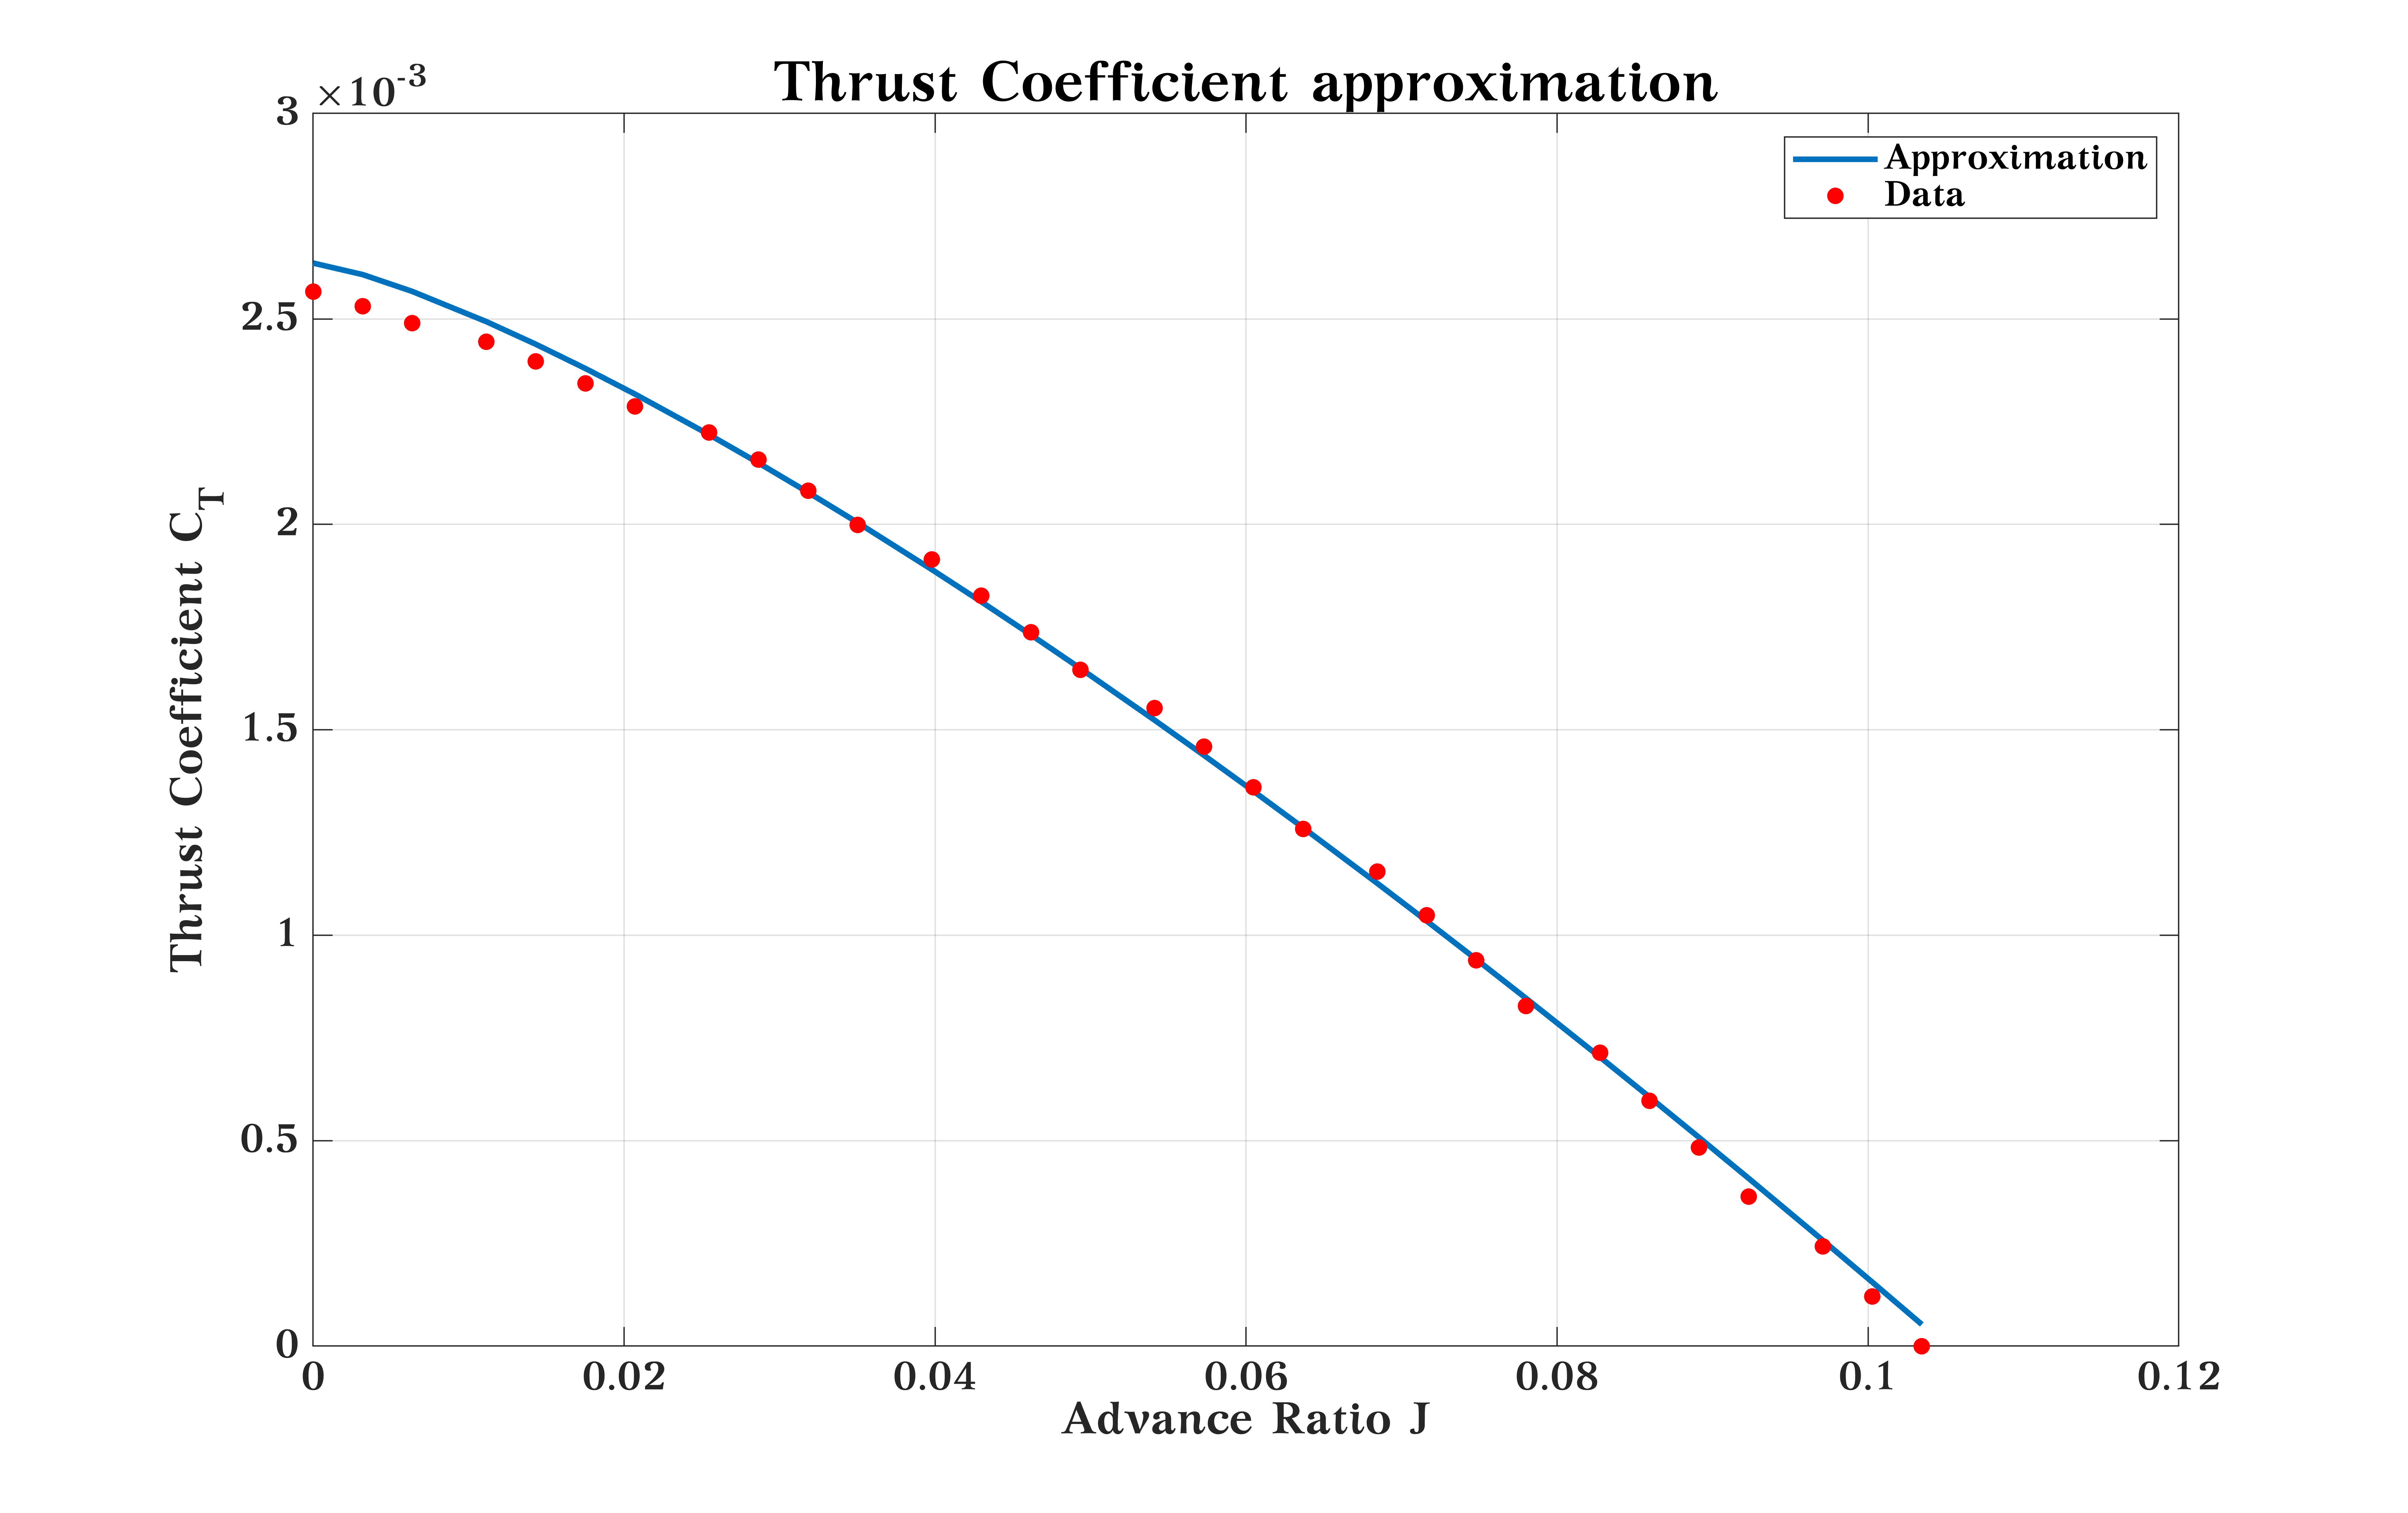
\includegraphics[width=\textwidth]{Propeller/fig_CT_J.png}
        \caption{Σύγκριση Συντελεστή Ώθησης}\label{fig_CT}
    \end{minipage}
    \quad
    \begin{minipage}[t]{0.48\linewidth}
        \centering
        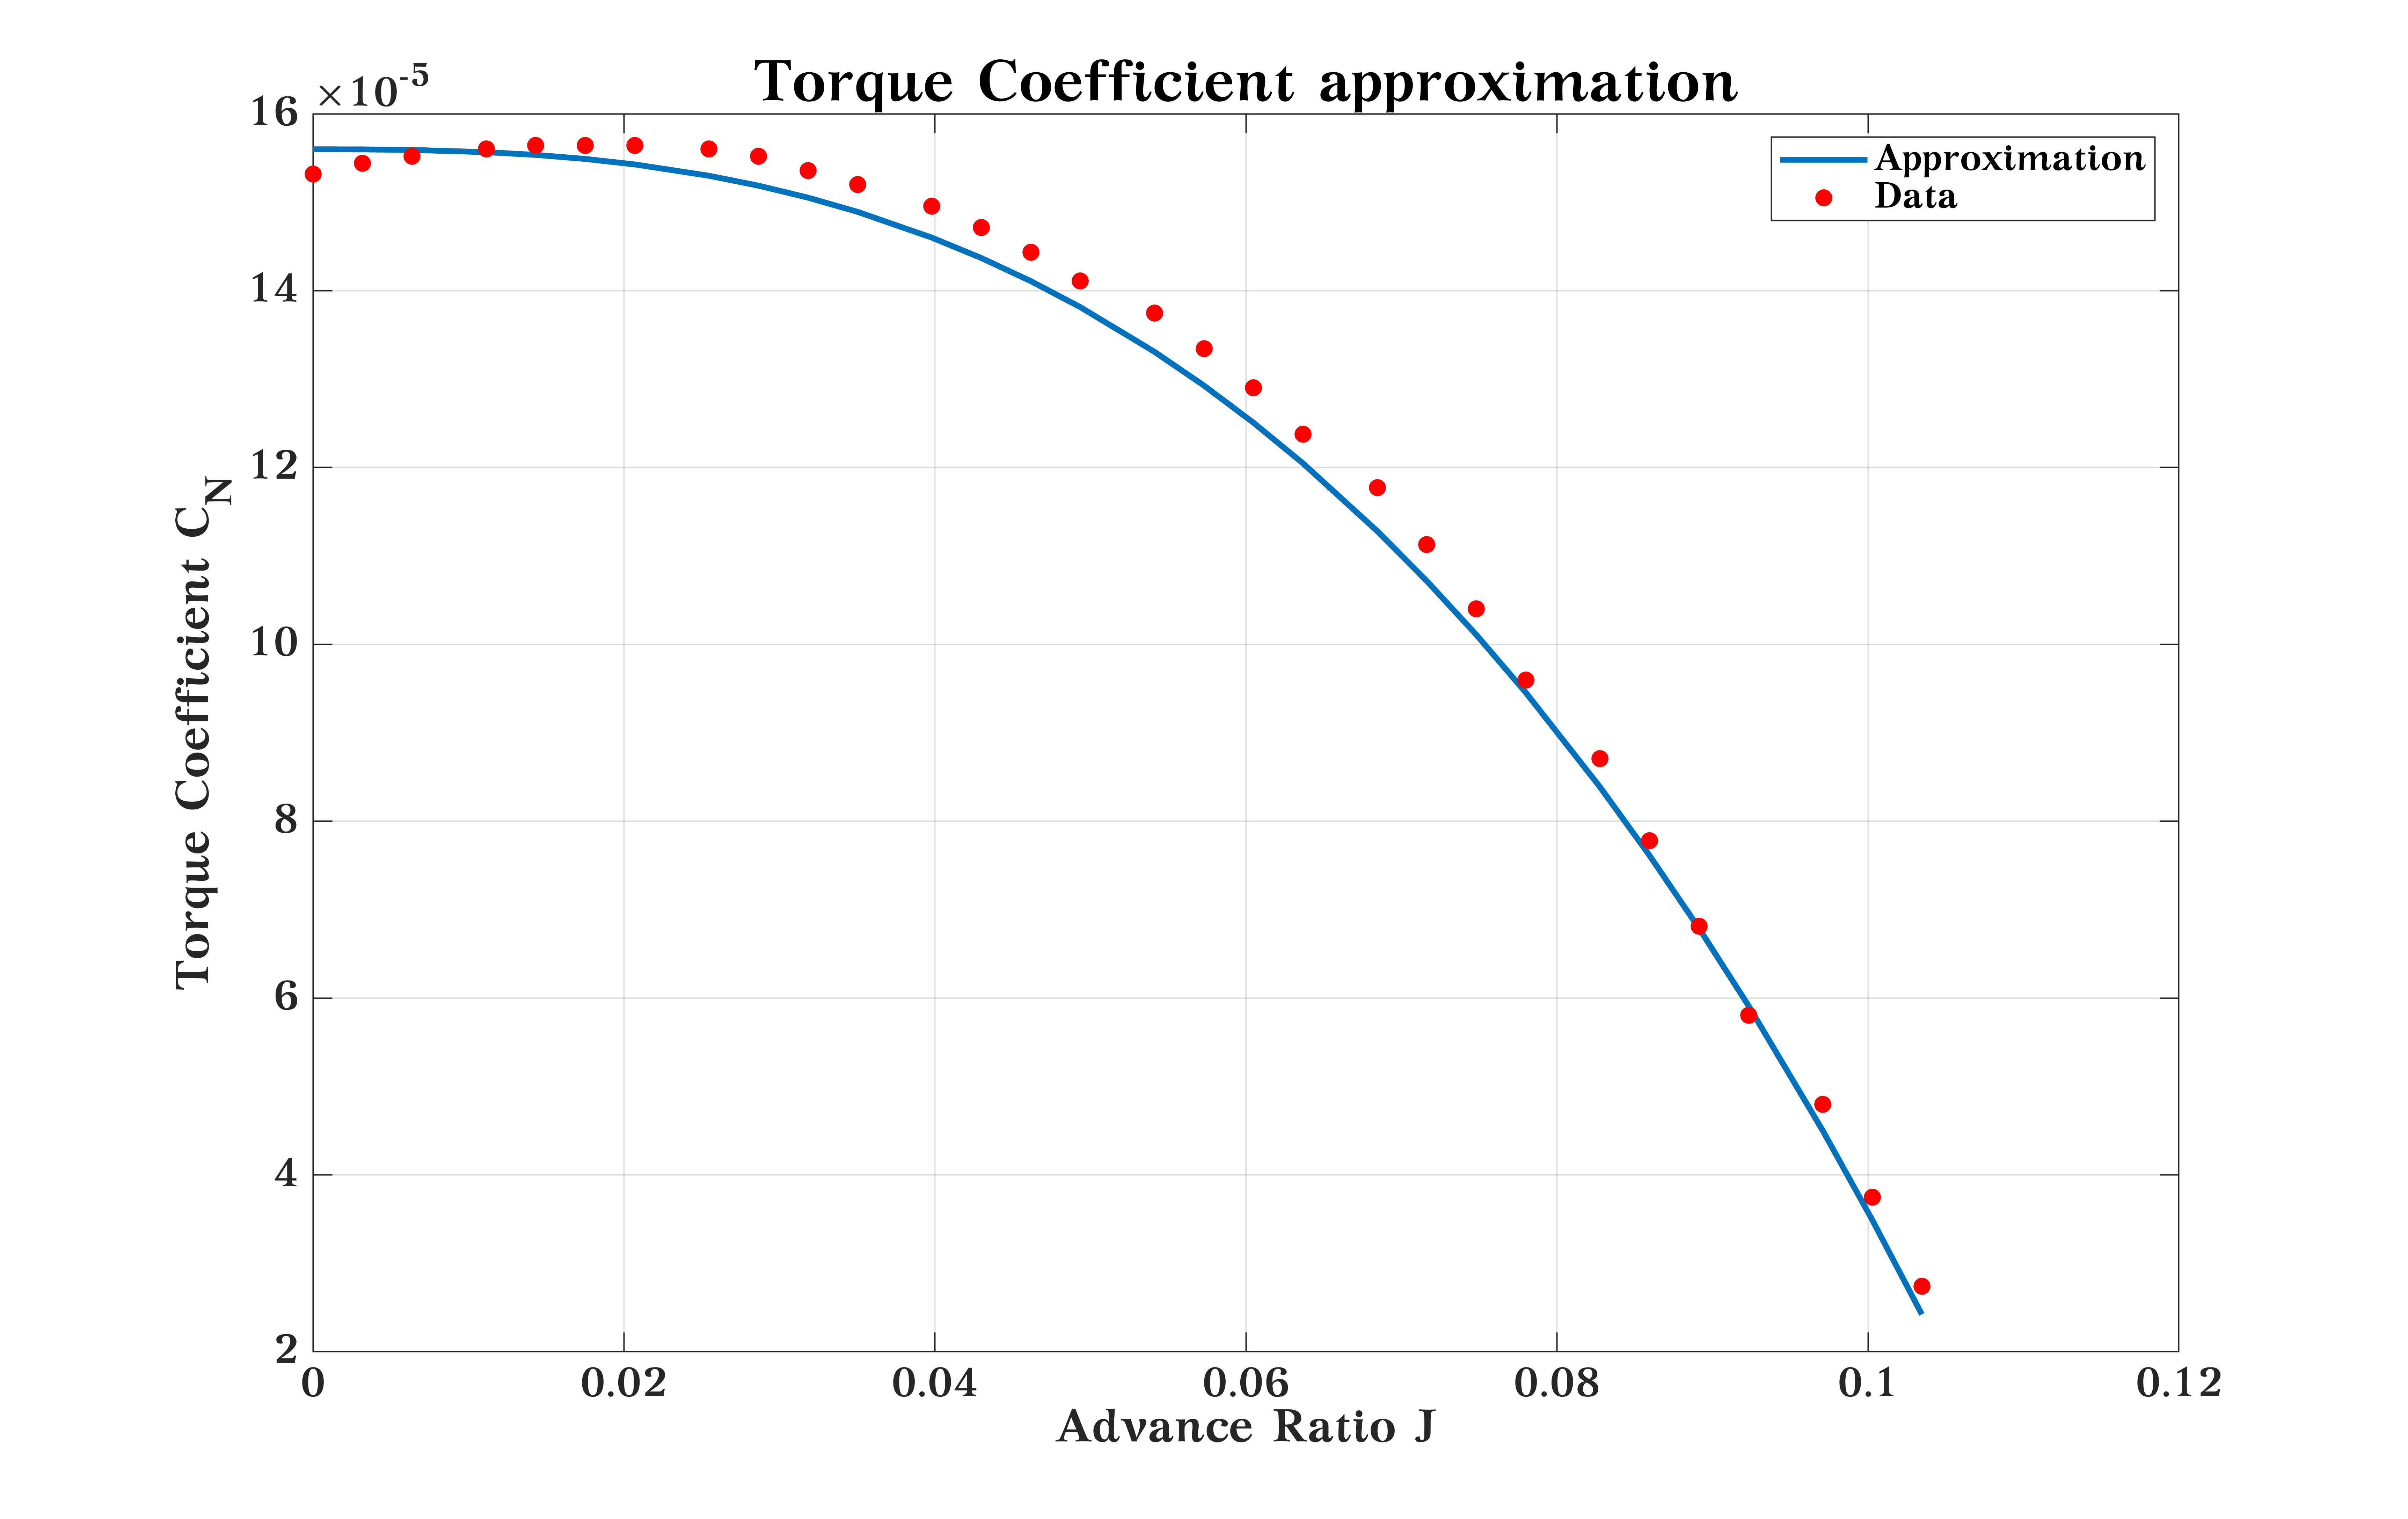
\includegraphics[width=\textwidth]{Propeller/fig_CN_J.png}
        \caption{Σύγκριση Συντελεστή Ροπής}\label{fig_CN}
    \end{minipage}
\end{figure}

Οι προσεγγιστικές σχέσεις των συντελεστών ώθησης και ροπής έχουν μορφή
\begin{gather*}
    C_T = \alpha_T J^{d_T} + \beta_T \\
    C_N = \alpha_N J^{d_N} + \beta_N.
\end{gather*}

Με την εύρεση των προσεγγιστικών σχέσεων, μπορεί να υπολογιστεί η δύναμη πρόωσης
και η ροπή αντίστασης των ελίκων (χρησιμοποιώντας τις εξισώσεις της 
μοντελοποίησης), γνωρίζοντας την γωνιακή τους ταχύτητα και την σχετική ταχύτητα 
του αεροχήματος προς τον άνεμο. Οι εξισώσεις μοντελοποίησης παίρνουν μορφή
\begin{gather*}
    T = \alpha_T \rho D^{4 - d_t} n^{2-d_t} V^{d_T} + \beta_T \rho D^4 n^2\\
    N = \alpha_N \rho D^{5 - d_N} n^{2-d_N} V^{d_N} + \beta_T \rho D^5 n^2.
\end{gather*}

Στα τρισδιάστατα διαγράμματα (\ref{surf_T}), (\ref{surf_N}) παρουσιάζεται η 
σύγκριση των δεδομένων της δύναμης πρόωσης και ροπής των ελίκων που παρέχονται 
από τον κατασκευαστή και τα αποτελέσματα από την μοντελοποίηση. Τα αποτελέσματα 
δίνονται για διαφορετικές γωνιακές ταχύτητες και σχετικές ταχύτητες του 
αεροχήματος. Οι γωνιακές ταχύτητες που θα λειτουργούν οι κινητήρες δεν θα 
ξεπερνάνε τα $1500 rad/s$ και όπως φαίνεται και στο διάγραμμα, σε εκείνη την 
περιοχή η προσέγγιση είναι ικανοποιητική.

\begin{figure}[hbt!]
    \centering
    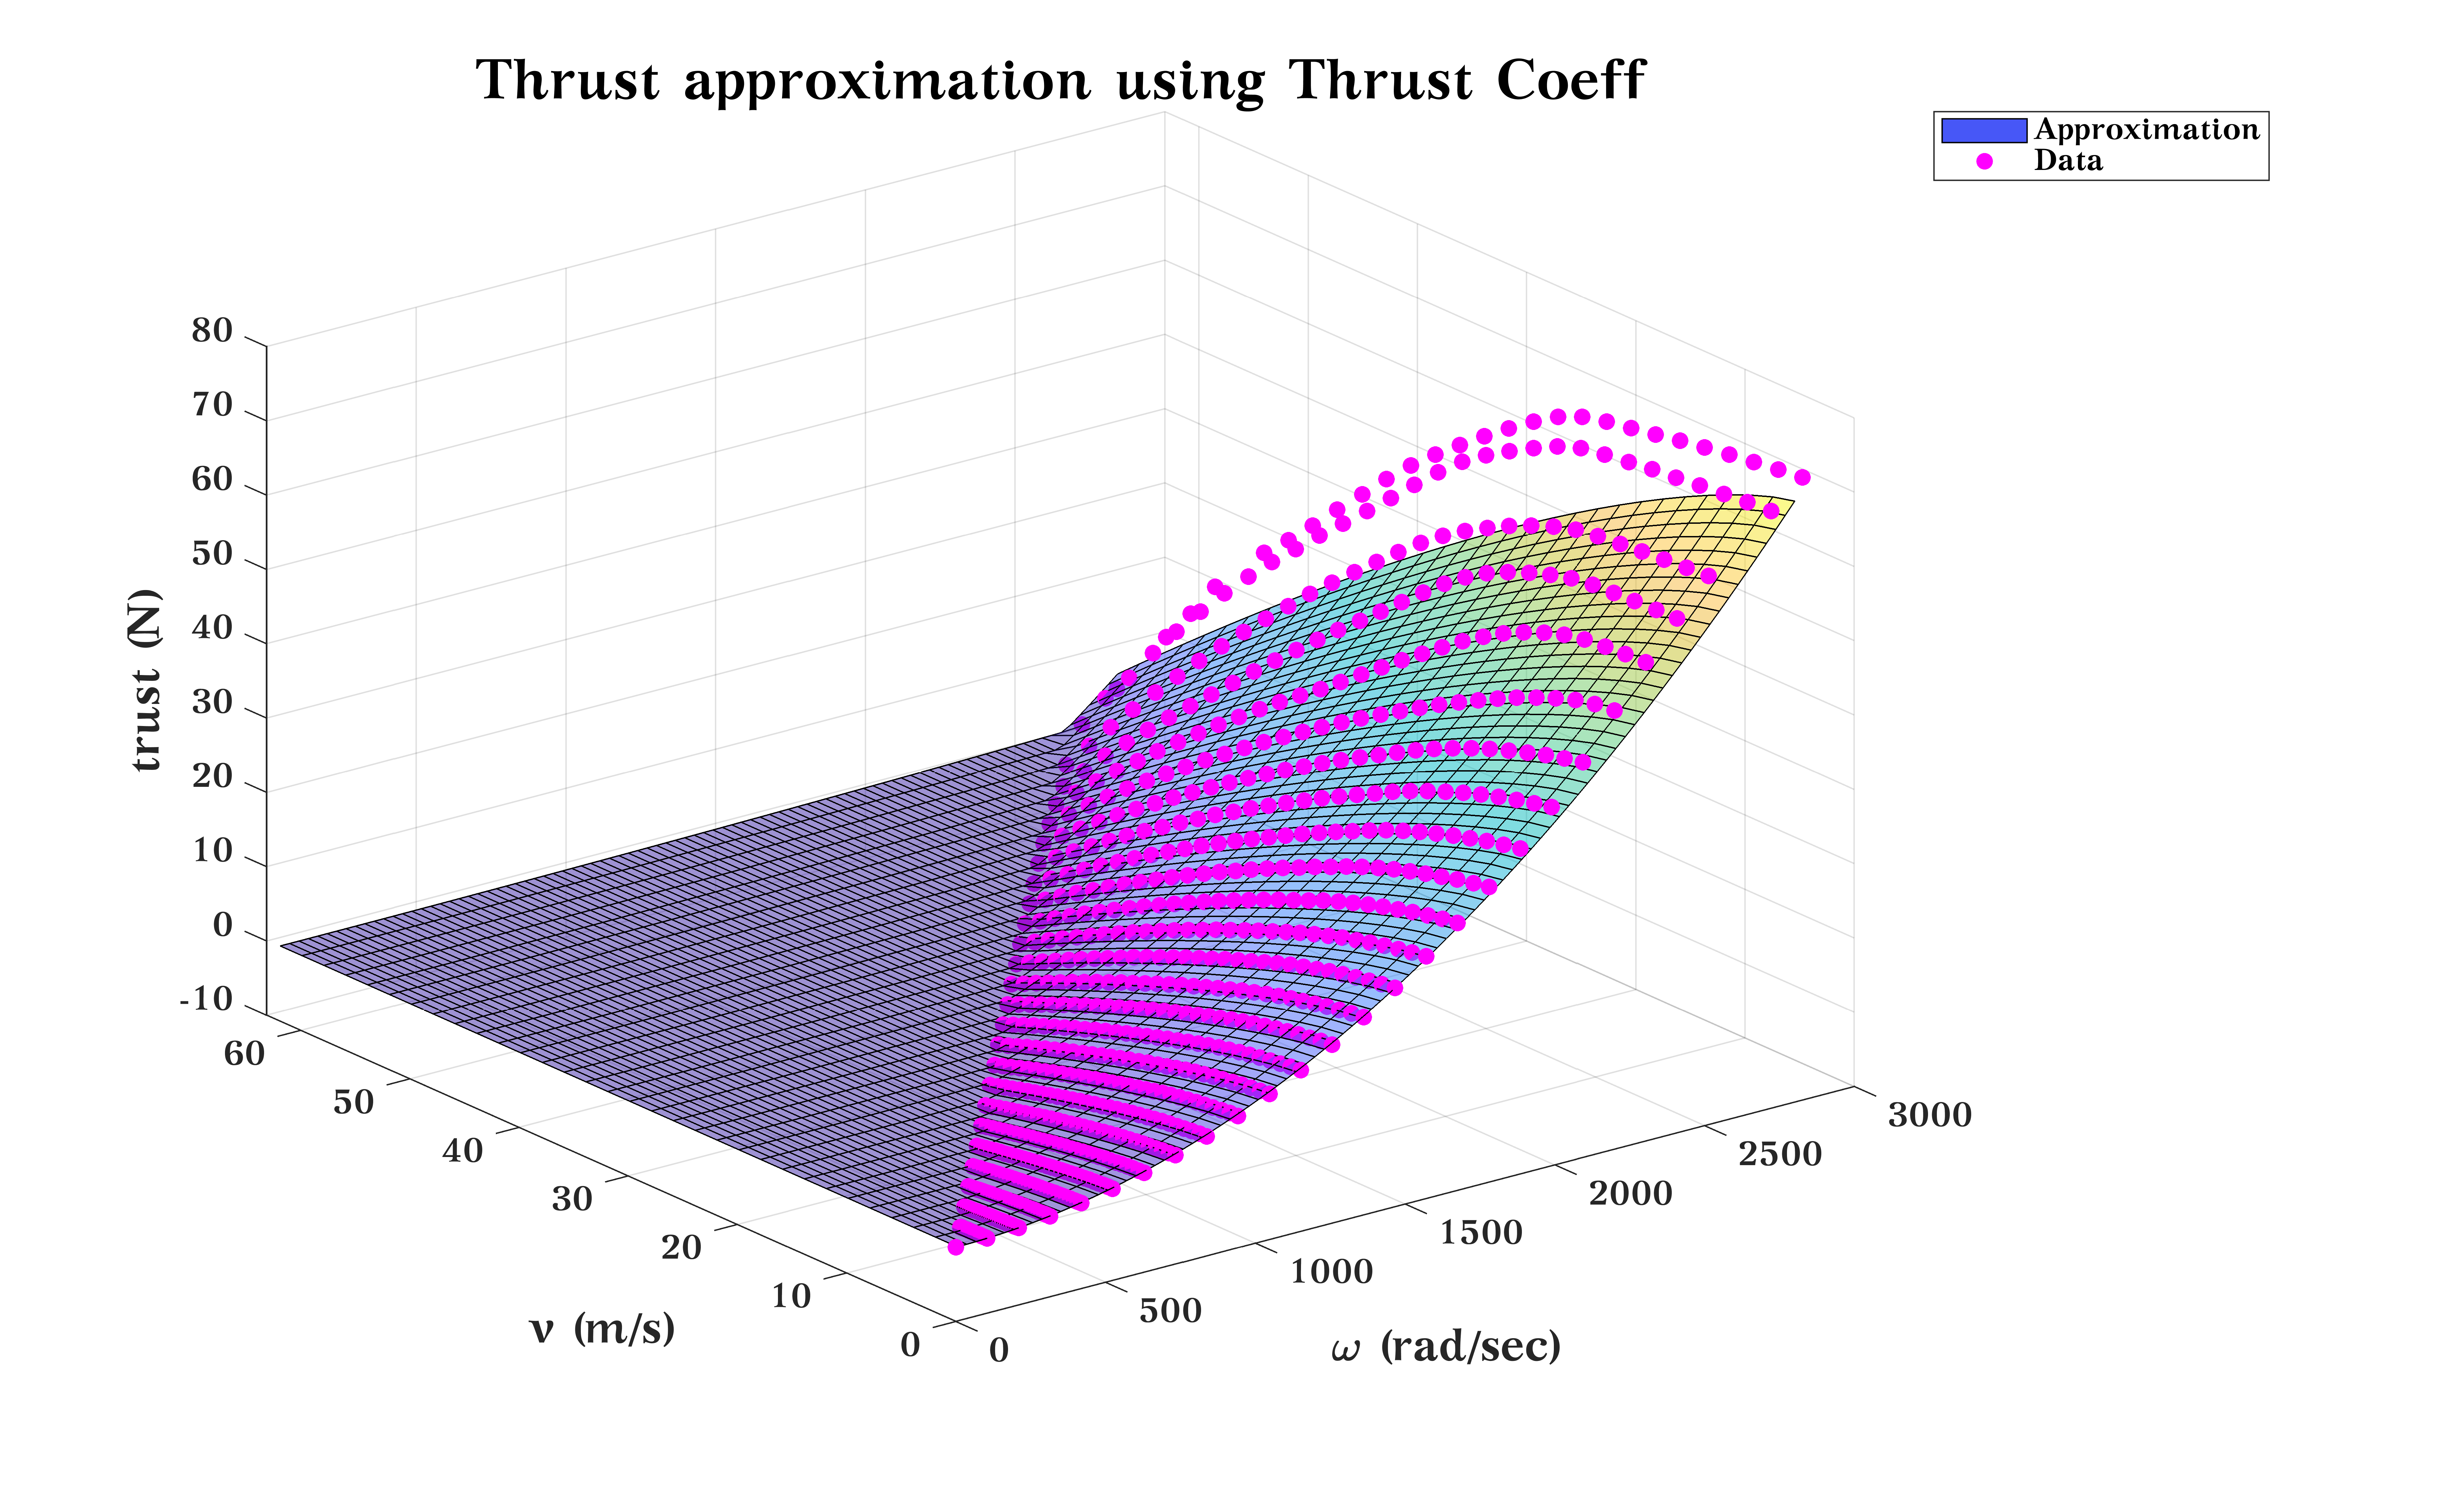
\includegraphics[scale=0.45]{Propeller/fig_surf_T.png}
    \caption{Σύγκριση Δύναμης Ώθησης}\label{surf_T}
\end{figure}

\begin{figure}[H]
    \centering
    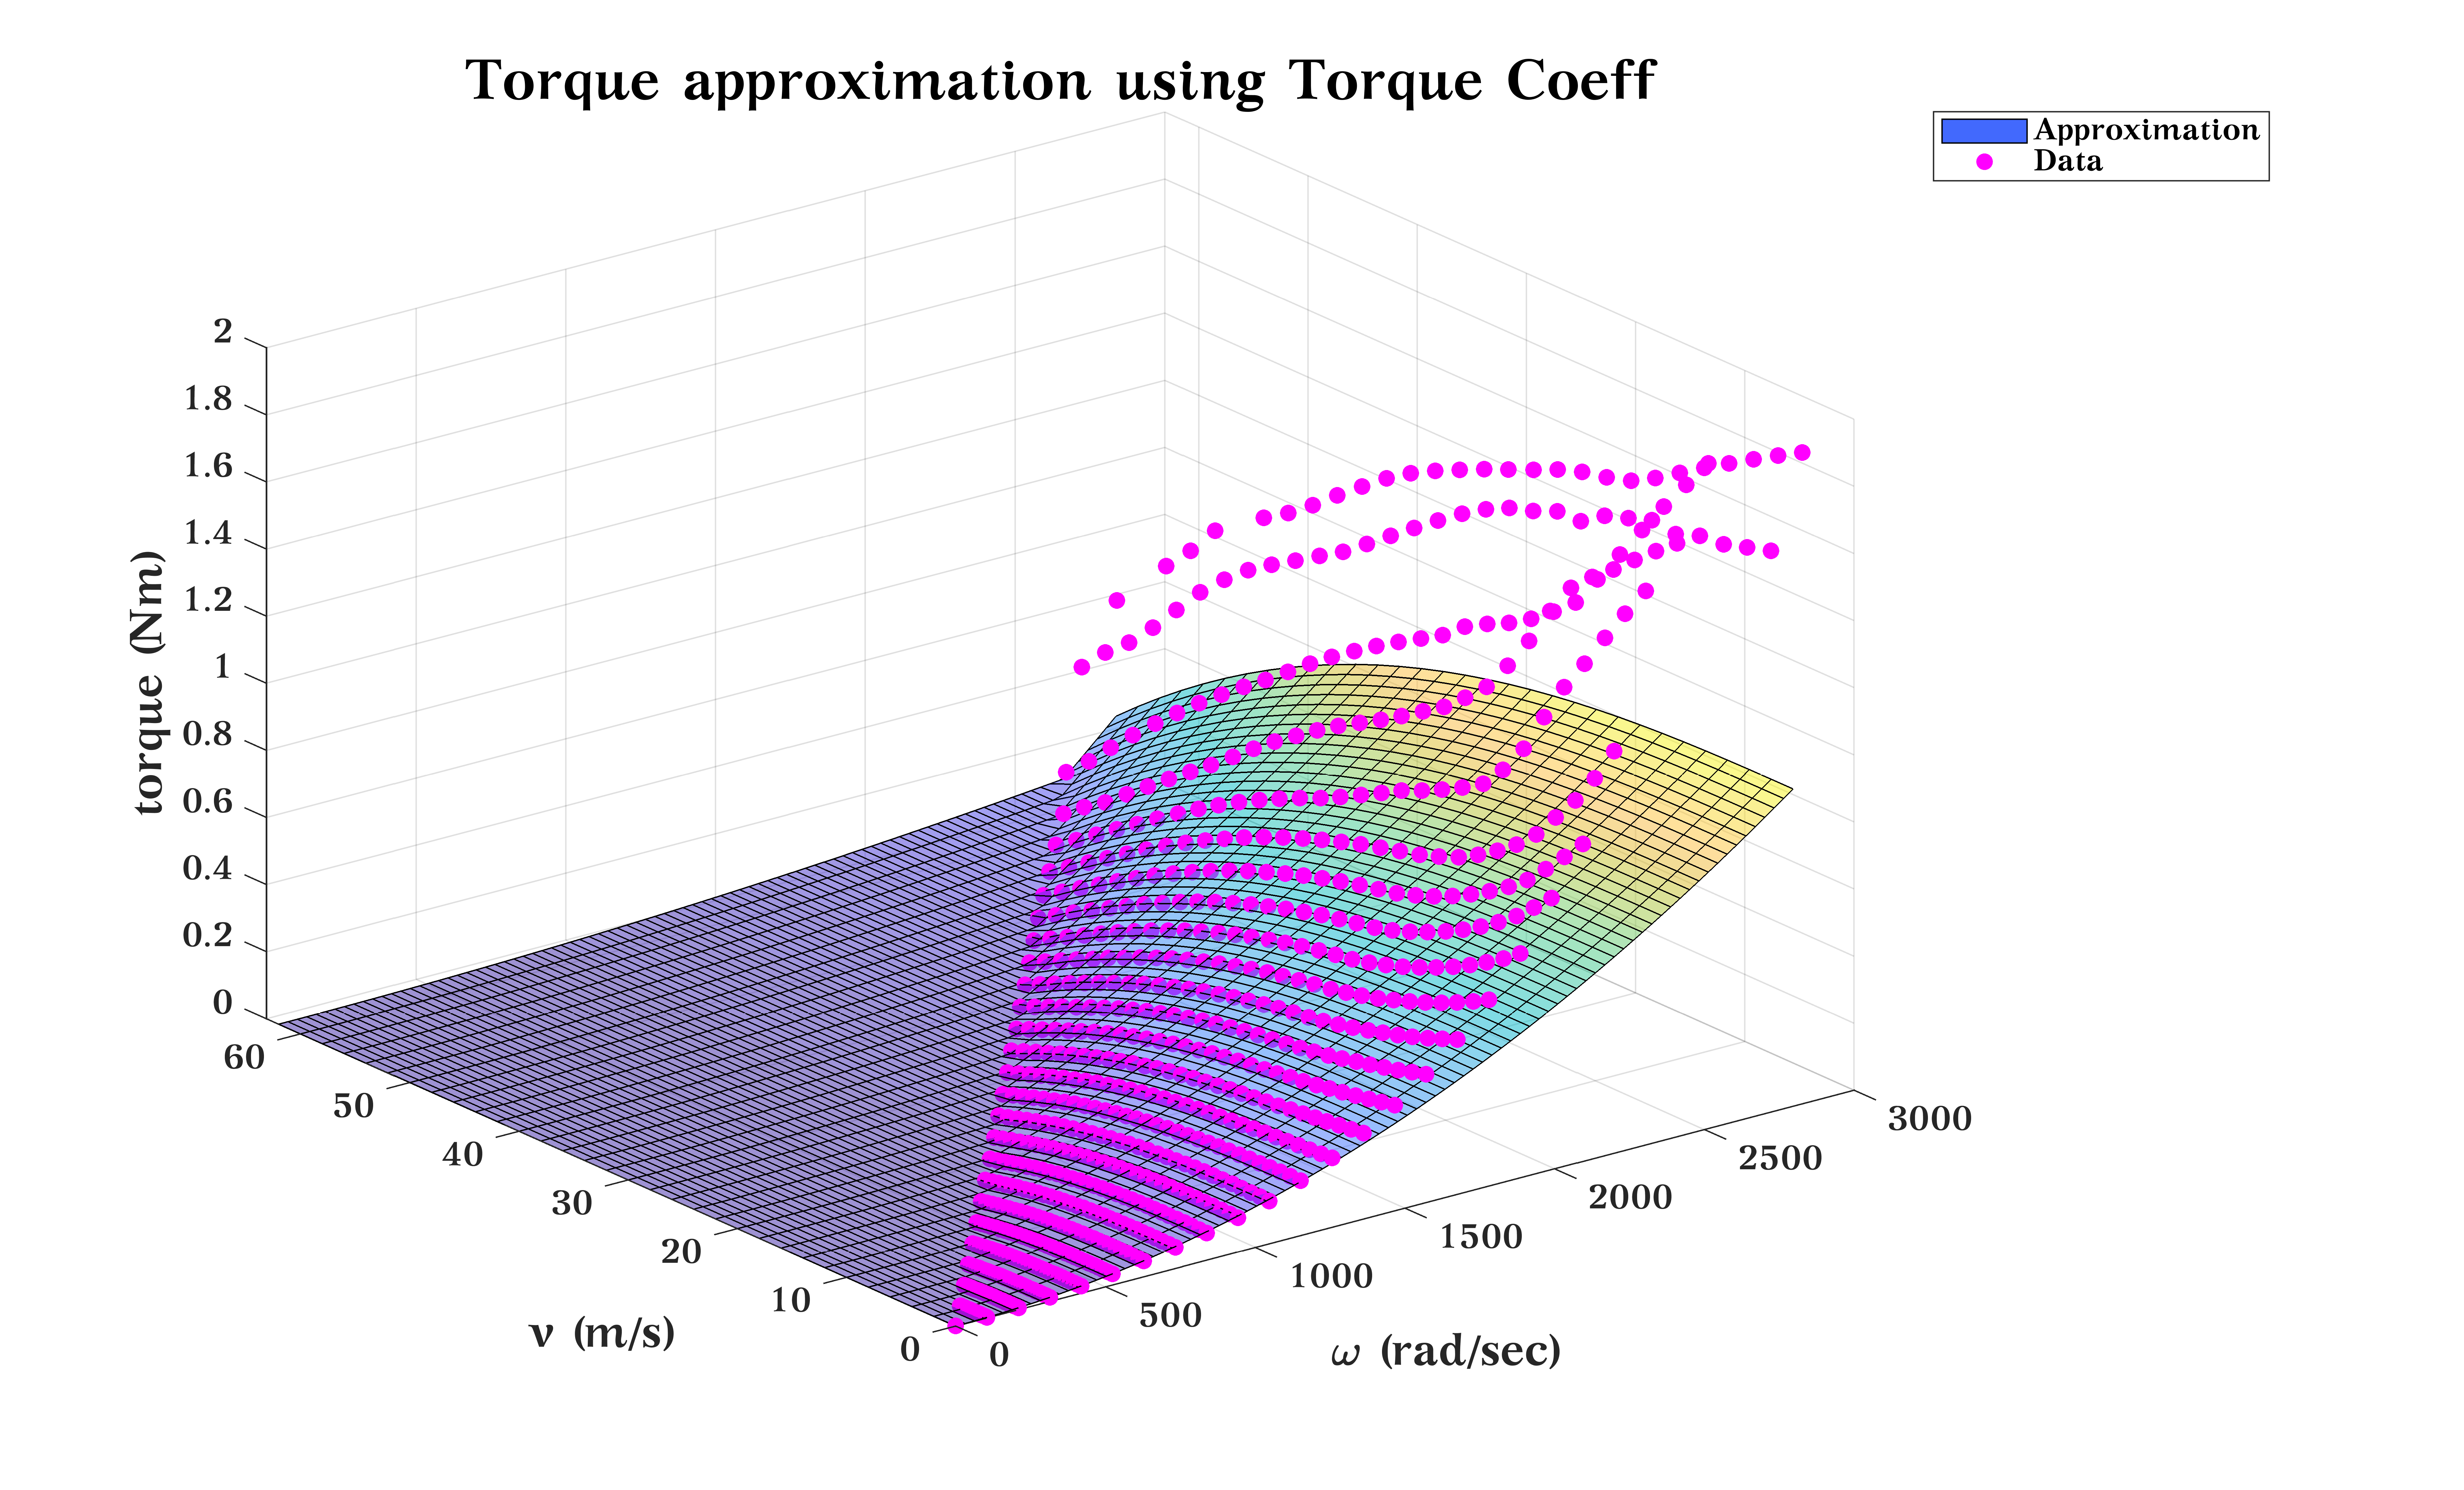
\includegraphics[scale=0.45]{Propeller/fig_surf_N.png}
    \caption{Σύγκριση Ροπής Αντίδρασης}\label{surf_N}
\end{figure}

\subsubsection{Χαρακτηρισμός Φορτίου Έλικας}
Στόχος της ενότητας είναι ο χαρακτηρισμός των παραγόμενων δυνάμεων \tl{T, N}, 
που, σε αντίθεση με την προηγούμενη αναλυτική μοντελοποίηση, θέτει τις δυνάμεις 
σε μορφή διαχειρίσιμη για την σύνθεση της αφινικής δομής. Για το χαρακτηρισμό 
του παραγόμενου φορτίου μιας έλικας απαιτούνται δεδομένα, που περιγράφουν τη 
δύναμη ώθησης καθώς και τη ροπή αντίδρασης συναρτήσει της γωνιακής ταχύτητας του 
κινητήρα και την ταχύτητα ανέμου

\begin{align*}
    T(\omega, V) &= \alpha \omega^2 + \beta V^2 \\
    N(\omega, V) &= \gamma \omega^2 + \delta V^2.
\end{align*}


Όσον αφορά τη δύναμη ώθησης, ορίζεται η απεικόνιση 
\(T:[0, \infty) \times [0, \infty) \rightarrow [0, \infty) \) με 
\( T(\omega, V) = \alpha \omega ^2 + \beta V ^2  \). Για την ροπή αντίδρασης 
ορίζεται \(N:[0, \infty) \times [0, \infty) \rightarrow [0, \infty) \) με 
\( N(\omega, V) = \gamma \omega ^2 + \delta V ^2  \), όπου \(\alpha, \beta, 
\gamma, \delta\) σταθεροί συντελεστές. Η μορφή αυτή των απεικονίσεων αποτελεί
κοινή πρακτική στις προπέλες μικρού μεγέθους στη βιβλιογραφία. Μέλημα, τώρα, 
είναι να βρεθούν οι συντελεστές αυτοί οι οποίοι περιγράφουν βέλτιστα τα 
δεδομένα. Αυτό πραγματοποιείται με τη χρήση της μεθόδου ελαχίστων τετραγώνων.
Το πρόβλημα που τίθεται προς λύση είναι 
\begin{equation*}
    Ax = b,
\end{equation*} 
όπου το μητρώο $A \in \euclr{n \times 2}$ περιέχει τα τετράγωνα των 
$\omega, V$, το διάνυσμα $x \in \mathbb{R}^2$ περιέχει τους συντελεστές 
$\alpha, \beta$ και το διάνυσμα $b \in \mathbb{R}^n$ περιέχει τη δύναμη 
ώθησης. Όπου \(n\) το πλήθος των δεδομένων. Δηλαδή,
\begin{equation*}
    A = \begin{bmatrix}
            \omega_1 ^2 & V_1 ^2\\
            \omega_2 ^2 & V_2 ^2\\
            \vdots      & \vdots\\
            \omega_n ^2 & V_n ^2 
        \end{bmatrix}
    ,\qquad 
    x = \begin{pmatrix}
            \alpha\\\beta
        \end{pmatrix}
    ,\qquad
    x = \begin{pmatrix}
        T_1 \\
        T_2 \\
        \vdots\\
        T_n 
        \end{pmatrix}.
    \end{equation*} 

Το πρόβλημα αυτό όμως δεν έχει λύση, γι' αυτό αναζητείται το \(\widehat{x}\), 
για το οποίο θα ισχύει 
\begin{equation*}
    dist(b,A\widehat{x}) \le dist(b, Ax) \qquad \forall x\in \mathbb{R}^n.
\end{equation*}

Το \(\widehat{x}\) υπολογίζεται, έτσι ώστε το διάνυσμα \(A \widehat{x}\) να 
είναι η προβολή του διανύσματος \(b\) στο χώρο στηλών του μητρώου \(A\). Με 
αυτόν τον τρόπο 
\begin{equation*}
    \widehat{x} = (A^TA)^{-1} A^T b.
\end{equation*}

Το διάνυσμα \(\widehat{x}\) επιστρέφει τις τιμές των \(\alpha, \beta\) που
προσεγγίζουν βέλτιστα τα δεδομένα του κατασκευαστή. Τα αποτελέσματα που 
προέκυψαν από τη μέθοδο ελαχίστων τετραγώνων για τη δύναμη ώθησης φαίνονται στο 
σχήμα (\ref{th_app}).
\begin{figure}[H]
    \centering
    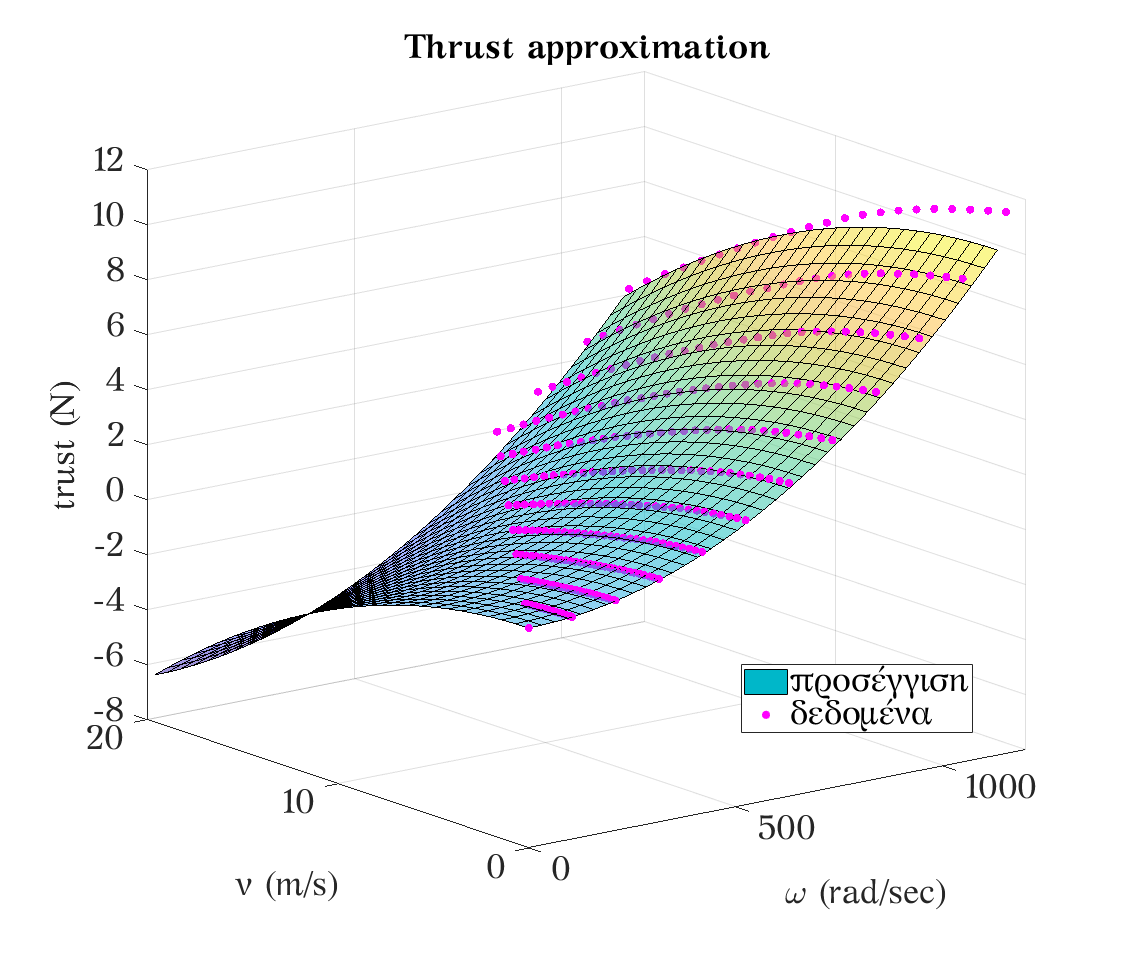
\includegraphics[width=0.5\textwidth]{Propeller/ThrustApproximation.png}
    \caption{Προσέγγιση δύναμης ώθησης}\label{th_app}
\end{figure}
Αντίστοιχα για την προσέγγιση της ροπής αντίδρασης μέσω της ίδιας μεθόδου 
προκύπτει το αποτέλεσμα του σχήματος (\ref{tq_app}).
\begin{figure}[H]
    \centering
    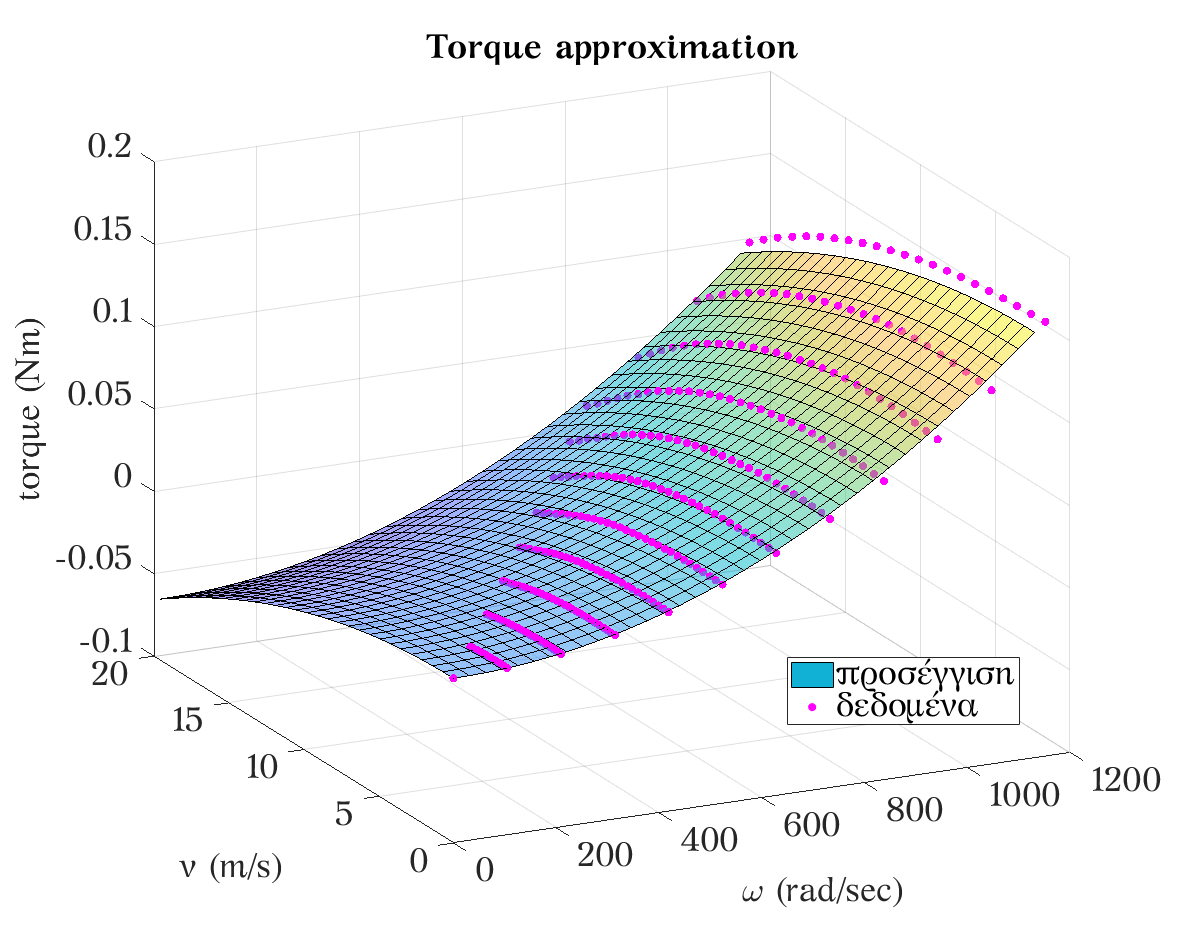
\includegraphics[width=0.5\textwidth]{Propeller/TorqueApproximation.png}
    \caption{Προσέγγιση ροπής αντίδρασης}\label{tq_app}
\end{figure}

Καθώς η αιώρηση του αεροχήματος περιορίζεται σε χαμηλές ταχύτητες πτήσης, ο όρος
που επηρεάζει σημαντικά τα φορτία είναι αυτός της γωνιακής ταχύτητας. Έτσι, 
είναι δόκιμο να απαλειφθεί ο όρος που σχετίζεται με την ταχύτητα ανέμου, δηλαδή 
ως απεικόνιση των φορτίων να χρησιμοποιηθεί η προβολή των συναρτήσεων \(T, N\) 
στη γωνιακή ταχύτητα. Οι προβολές που προκύπτουν θα έχουν το μορφή 
\(\widehat{T} = \alpha \omega^2\) και \(\widehat{N} = \gamma \omega^2\).
Στο αερόχημα, όπου χρησιμοποιούνται δύο είδη ελίκων, αυτή η διαδικασία γίνεται 
δύο φορές, έτσι ορίζονται οι συναρτήσεις της δύναμης ώθησης και της ροπής 
αντίδρασης για τις δύο έλικες. Για την έλικα, που χρησιμοποιείται στους 
εμπρόσθιους κινητήρες, ορίζονται οι απεικονίσεις
\(p_T:[0, \infty) \rightarrow [0, \infty) \) και 
\(p_N:[0, \infty) \rightarrow [0, \infty) \) με \(p_T = p_1 \omega ^2\) και
\(p_N = p_2 \omega ^2\).
Για την οπίσθια έλικα ορίζονται
\(q_T:[0, \infty) \rightarrow [0, \infty) \) και 
\(q_N:[0, \infty) \rightarrow [0, \infty) \) με \(q_T = p_3 \omega ^2\) και
\(q_N = p_4 \omega ^2\).   

Οι έλικες, οι οποίες επιλέχθηκαν στην παρούσα εργασία, είναι οι \tl{Master 
AirScrew} διάστασης $9\times 4$ για τους δύο εμπρόσθιους κινητήρες, ενώ για τον 
πισινό κινητήρα επιλέχθηκε η έλικα \tl{APCProp} διάστασης $10 \times 4.5$.

\begin{figure}[hbt!]
    \begin{subfigure}{0.48\textwidth}
        \centering
        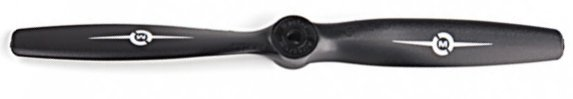
\includegraphics[width=\textwidth]{Propeller/Master_Airsrew_9x4.jpg} 
        \caption{\tl{Master Airscrew 9x4}}
    \end{subfigure}
    \begin{subfigure}{0.48\textwidth}
        \centering
        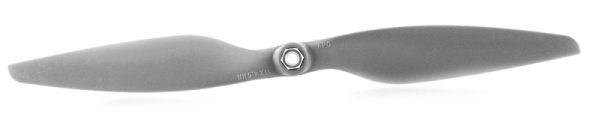
\includegraphics[width=\textwidth]{Propeller/APCProp_10x45MR.png}
        \caption{\tl{APC Propellers 10x4.5}}
    \end{subfigure}
    \caption{Έλικες}
    \label{fig:image2}
\end{figure}

Τέλος για την επιβεβαίωση των στοιχείων που προσφέρει ο κατασκευαστής 
πραγματοποιήθηκαν μετρήσεις της παραγόμενης ώθησης για τις έλικες που  
χρησιμοποιούνται. Οι μετρήσεις έγιναν υπό στατικές συνθήκες (μηδενική σχετική 
ταχύτητα ανέμου) και τα αποτελέσματα έδειξαν σύγκλιση στις τιμές του 
κατασκευαστή. Για τις ανάγκες των μετρήσεων χρησιμοποιήθηκε το ζυγιστικό 
όργανο \tl{Load-Cell 10kg (TAL220)}, o μικροελεγκτής \tl{Arduino UNO} καθώς και 
το απαιτούμενο σύστημα για την οδήγηση ενός κινητήρα στις απαιτούμενες στροφές. 
Ο μικροελεγκτής προγραμματίστηκε σε γλώσσα προγραμματισμού \tl{C/C++}.
\begin{figure}[H]
    \centering
    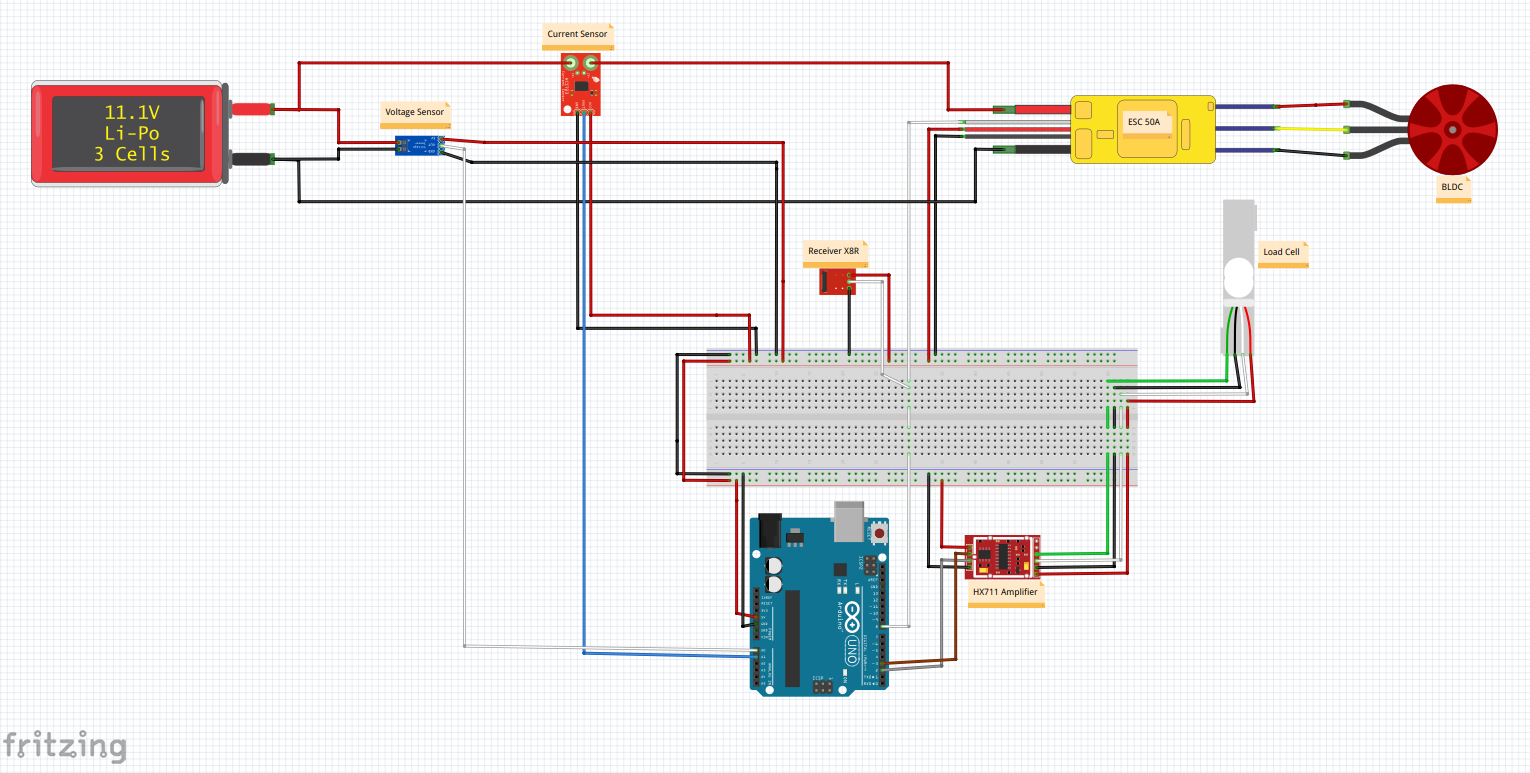
\includegraphics[width=\textwidth]{Propeller/schematic.png} 
    \caption{Σχηματική αναπαράσταση μετριτικής διάταξης}
\end{figure}
